\documentclass[10pt]{beamer}
\usepackage[utf8]{inputenc}
\usepackage{tikz, pgfplots}
\pgfplotsset{compat=1.18}
\usetikzlibrary{positioning}
\usetikzlibrary{trees}
\usetikzlibrary{shapes.geometric, arrows.meta, positioning}
\usepackage{xcolor}
\usepackage{graphicx}
\usepackage{subcaption}
\usepackage{hyperref} 
\usepackage{colortbl} % Required for \rowcolor
\usepackage{animate}
\usepackage[T1]{fontenc}
\usepackage{amsmath, amsfonts, amssymb}
\usepackage{cancel}
\usepackage[french]{babel}
\usepackage[normalem]{ulem}
\usepackage{multicol}

\setlength{\columnsep}{1cm}        % khoảng cách giữa 2 cột
\setlength{\columnseprule}{2pt}    % độ rộng vạch đứng
\renewcommand{\columnseprulecolor}{\color{gray}} % màu vạch

% Theme và màu sắc cho beamer
\usetheme{AnnArbor}
\usecolortheme{seahorse}

% Định nghĩa và thiết lập màu sắc chung
\definecolor{mydarkblue}{RGB}{0,51,102}
\setbeamercolor{structure}{fg=mydarkblue}
\setbeamercolor{frametitle}{bg=mydarkblue, fg=white}
\setbeamercolor{title}{fg=mydarkblue}
\setbeamercolor{item}{fg=mydarkblue}
\setbeamercolor{block title}{bg=mydarkblue, fg=white}
\setbeamercolor{block body}{bg=white, fg=black}
\setbeamercolor{section in toc}{fg=mydarkblue}
\setbeamercolor{subsection in toc}{fg=mydarkblue}
\setbeamercolor{caption name}{fg=mydarkblue}
\setbeamercolor{author}{fg=mydarkblue}
\setbeamercolor{date}{fg=mydarkblue}
\setbeamercolor{institute}{fg=mydarkblue}
\setbeamertemplate{caption}[numbered]
\usepackage{multirow}
\title{Rapport Hebdo}
\author{Viet Anh Quach}
\institute{3SR}
\date{\today}

\begin{document}

% \begin{frame}
%     \titlepage
% \end{frame}

% \section{Étude bibliographie}

% \section{DEM}

% % 03102025
% \begin{frame}{Article Stress-strain behavior of sand at high strain rates (Mehdi Omidvar et al,2012)}
%             \begin{figure}[h]
%                 \centering
%                 \scalebox{0.4}{\includegraphics{StrainRate.png}}
%             \end{figure}
%             "Under HSR loading, there is not enough time for strain energy
% accumulation, which prohibits crushing and promotes
% rolling-rearrangement resulting in a higher resistance to shear"
% \end{frame}


% \begin{frame}{Trouver le régime de l'état critique}
%     \begin{columns}
%                 \begin{column}{0.5\textwidth}
%             \begin{figure}
%                 \centering
%                 \scalebox{0.5}{% GNUPLOT: LaTeX picture with Postscript
\begingroup
  \makeatletter
  \providecommand\color[2][]{%
    \GenericError{(gnuplot) \space\space\space\@spaces}{%
      Package color not loaded in conjunction with
      terminal option `colourtext'%
    }{See the gnuplot documentation for explanation.%
    }{Either use 'blacktext' in gnuplot or load the package
      color.sty in LaTeX.}%
    \renewcommand\color[2][]{}%
  }%
  \providecommand\includegraphics[2][]{%
    \GenericError{(gnuplot) \space\space\space\@spaces}{%
      Package graphicx or graphics not loaded%
    }{See the gnuplot documentation for explanation.%
    }{The gnuplot epslatex terminal needs graphicx.sty or graphics.sty.}%
    \renewcommand\includegraphics[2][]{}%
  }%
  \providecommand\rotatebox[2]{#2}%
  \@ifundefined{ifGPcolor}{%
    \newif\ifGPcolor
    \GPcolortrue
  }{}%
  \@ifundefined{ifGPblacktext}{%
    \newif\ifGPblacktext
    \GPblacktextfalse
  }{}%
  % define a \g@addto@macro without @ in the name:
  \let\gplgaddtomacro\g@addto@macro
  % define empty templates for all commands taking text:
  \gdef\gplbacktext{}%
  \gdef\gplfronttext{}%
  \makeatother
  \ifGPblacktext
    % no textcolor at all
    \def\colorrgb#1{}%
    \def\colorgray#1{}%
  \else
    % gray or color?
    \ifGPcolor
      \def\colorrgb#1{\color[rgb]{#1}}%
      \def\colorgray#1{\color[gray]{#1}}%
      \expandafter\def\csname LTw\endcsname{\color{white}}%
      \expandafter\def\csname LTb\endcsname{\color{black}}%
      \expandafter\def\csname LTa\endcsname{\color{black}}%
      \expandafter\def\csname LT0\endcsname{\color[rgb]{1,0,0}}%
      \expandafter\def\csname LT1\endcsname{\color[rgb]{0,1,0}}%
      \expandafter\def\csname LT2\endcsname{\color[rgb]{0,0,1}}%
      \expandafter\def\csname LT3\endcsname{\color[rgb]{1,0,1}}%
      \expandafter\def\csname LT4\endcsname{\color[rgb]{0,1,1}}%
      \expandafter\def\csname LT5\endcsname{\color[rgb]{1,1,0}}%
      \expandafter\def\csname LT6\endcsname{\color[rgb]{0,0,0}}%
      \expandafter\def\csname LT7\endcsname{\color[rgb]{1,0.3,0}}%
      \expandafter\def\csname LT8\endcsname{\color[rgb]{0.5,0.5,0.5}}%
    \else
      % gray
      \def\colorrgb#1{\color{black}}%
      \def\colorgray#1{\color[gray]{#1}}%
      \expandafter\def\csname LTw\endcsname{\color{white}}%
      \expandafter\def\csname LTb\endcsname{\color{black}}%
      \expandafter\def\csname LTa\endcsname{\color{black}}%
      \expandafter\def\csname LT0\endcsname{\color{black}}%
      \expandafter\def\csname LT1\endcsname{\color{black}}%
      \expandafter\def\csname LT2\endcsname{\color{black}}%
      \expandafter\def\csname LT3\endcsname{\color{black}}%
      \expandafter\def\csname LT4\endcsname{\color{black}}%
      \expandafter\def\csname LT5\endcsname{\color{black}}%
      \expandafter\def\csname LT6\endcsname{\color{black}}%
      \expandafter\def\csname LT7\endcsname{\color{black}}%
      \expandafter\def\csname LT8\endcsname{\color{black}}%
    \fi
  \fi
    \setlength{\unitlength}{0.0500bp}%
    \ifx\gptboxheight\undefined%
      \newlength{\gptboxheight}%
      \newlength{\gptboxwidth}%
      \newsavebox{\gptboxtext}%
    \fi%
    \setlength{\fboxrule}{0.5pt}%
    \setlength{\fboxsep}{1pt}%
    \definecolor{tbcol}{rgb}{1,1,1}%
\begin{picture}(7200.00,5040.00)%
    \gplgaddtomacro\gplbacktext{%
      \csname LTb\endcsname%%
      \put(682,704){\makebox(0,0)[r]{\strut{}$-5$}}%
      \csname LTb\endcsname%%
      \put(682,1527){\makebox(0,0)[r]{\strut{}$0$}}%
      \csname LTb\endcsname%%
      \put(682,2350){\makebox(0,0)[r]{\strut{}$5$}}%
      \csname LTb\endcsname%%
      \put(682,3173){\makebox(0,0)[r]{\strut{}$10$}}%
      \csname LTb\endcsname%%
      \put(682,3996){\makebox(0,0)[r]{\strut{}$15$}}%
      \csname LTb\endcsname%%
      \put(682,4819){\makebox(0,0)[r]{\strut{}$20$}}%
      \csname LTb\endcsname%%
      \put(814,484){\makebox(0,0){\strut{}$0$}}%
      \csname LTb\endcsname%%
      \put(1469,484){\makebox(0,0){\strut{}$5$}}%
      \csname LTb\endcsname%%
      \put(2124,484){\makebox(0,0){\strut{}$10$}}%
      \csname LTb\endcsname%%
      \put(2779,484){\makebox(0,0){\strut{}$15$}}%
      \csname LTb\endcsname%%
      \put(3435,484){\makebox(0,0){\strut{}$20$}}%
      \csname LTb\endcsname%%
      \put(4090,484){\makebox(0,0){\strut{}$25$}}%
      \csname LTb\endcsname%%
      \put(4745,484){\makebox(0,0){\strut{}$30$}}%
      \csname LTb\endcsname%%
      \put(5400,484){\makebox(0,0){\strut{}$35$}}%
      \csname LTb\endcsname%%
      \put(6055,484){\makebox(0,0){\strut{}$40$}}%
      \put(6187,704){\makebox(0,0)[l]{\strut{}$-5$}}%
      \put(6187,1527){\makebox(0,0)[l]{\strut{}$0$}}%
      \put(6187,2350){\makebox(0,0)[l]{\strut{}$5$}}%
      \put(6187,3173){\makebox(0,0)[l]{\strut{}$10$}}%
      \put(6187,3996){\makebox(0,0)[l]{\strut{}$15$}}%
      \put(6187,4819){\makebox(0,0)[l]{\strut{}$20$}}%
      \put(1862,4325){\makebox(0,0)[r]{\strut{}hpd}}%
      \put(1862,4161){\makebox(0,0)[r]{\strut{}gd}}%
    }%
    \gplgaddtomacro\gplfronttext{%
      \csname LTb\endcsname%%
      \put(209,2761){\rotatebox{-270}{\makebox(0,0){\strut{}$\varepsilon_{v}(hpd) (\%)$}}}%
      \put(6693,2761){\rotatebox{-270}{\makebox(0,0){\strut{}$\varepsilon_{v}(gd) (\%)$}}}%
      \put(3434,154){\makebox(0,0){\strut{}$\varepsilon_{yy} (\%)$}}%
    }%
    \gplbacktext
    \put(0,0){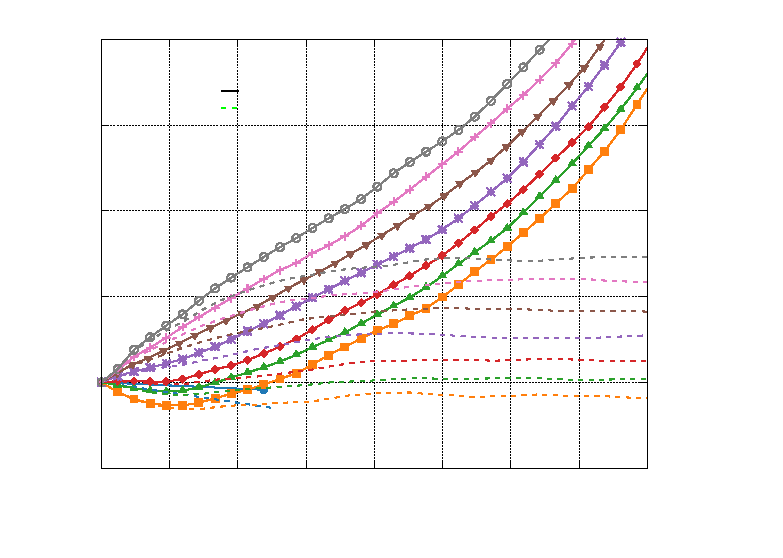
\includegraphics[width={360.00bp},height={252.00bp}]{Eyy_Ev}}%
    \gplfronttext
  \end{picture}%
\endgroup
}
%                 \caption{Déformation Volumique}
%             \end{figure}
%             \small
%             hpp: $\varepsilon_{yy} = \dfrac{\Delta h_{yy}}{h_{yy}^0}; \varepsilon_v = \varepsilon_{xx} + \varepsilon_{yy} + \varepsilon_{zz} $\\
%             gd: $\varepsilon_{yy} = \ln\left(\dfrac{h_{yy}}{h_{yy}^0}\right);  \varepsilon_v = \dfrac{\Delta V}{V_0}$;
%         \end{column}
%         \begin{column}{0.5\textwidth}
%             \begin{figure}
%                 \centering
%                 \scalebox{0.5}{\input{NombreCoordination.tex}}
%                 \caption{Nombre de Coordination}
%             \end{figure}
%             $Z = \dfrac{2N_{contact}}{N_{particule}}$; $I = \dfrac{v}{H_0}\sqrt{\dfrac{m}{P\overline{a}}}$
%         \end{column}
%     \end{columns}
% \end{frame}

% \begin{frame}{Trouver le régime de l'état critique}
%     \begin{columns}
%                 \begin{column}{0.5\textwidth}
%             \begin{figure}
%                 \centering
%                 \scalebox{0.5}{\input{Aleatoire.tex}}
%                 \caption{Nombre de Coordination}
%             \end{figure}
%             échantillon aléatoire par compression dans l'axe Z
%         \end{column}
%         \begin{column}{0.5\textwidth}
%             \begin{figure}
%                 \centering
%                 \scalebox{0.5}{\input{ComparerNP.tex}}
%                 \caption{Nombre de Particules}
%             \end{figure}
%         \end{column}
%     \end{columns}

% \end{frame}


\section{MPM}

\begin{frame}{État Rankine - Modèle}
	\begin{figure}
		\centering
		\includegraphics[height = 2.3cm]{activeRankine.pdf}
		\caption{Pression active:le mur s'éloigne du sol}
	\end{figure}
	\begin{figure}
		\centering
		\includegraphics[height = 2.3cm]{passiveRankine.pdf}
		\caption{Pression passive:le mur se rapproche du sol}
	\end{figure}
	Observer la pression sur le mur en bleu
\end{frame}


% \begin{frame}{Stabilisation - Théorie élastique}
% 	$E = 1e9\ Pa, \nu=0.2, \varphi=25^{\circ}, \psi=0^{\circ},c=0, PIC=99\%$
% 		\begin{figure}
% 			\centering
% 			\scalebox{0.35}{\input{ForceFond.tex}}
% 			\caption{La force au fond au repos}
% 		\end{figure}
		% à 1s, le modèle est bien stabilisé.\\
% 			\begin{align}
% 		\sigma_{yy} & = \rho \, g \, H = 2700 \cdot 9.81 \cdot 1 = 26487\ \text{Pa}                                                  \\[6pt]
% 		F_{yy}      & = \sigma_{yy} \cdot L = 26487 \cdot 3 = 79461\ \text{N}                                                        \\[6pt]
% 		\text{Modèle élastique: }K_0 &= \dfrac{\sigma_{xx}}{sigma_{yy}} = \dfrac{\nu}{1 - \nu}                                                                     \\[6pt]
% \end{align}
% \end{frame}

\begin{frame}{Stabilisation - Modèle avec des points fixées}
		\begin{figure}[h]
			\centering
			\begin{tikzpicture}

				% Đặt ảnh làm nền
				\node[anchor=south west, inner sep=0] (img) at (0,0)
				{\includegraphics[height=5cm]{ligneFix.png}};

				% Hệ toạ độ chuẩn hoá 0–1 theo ảnh
				\begin{scope}[x={(img.south east)}, y={(img.north west)}]
					% Vẽ hình chữ nhật màu đỏ
					\draw[red, thick] (0.465,0.3) rectangle (0.475,0.62);
					\draw[red, thick] (0.74,0.3) rectangle (0.75,0.62);
				\end{scope}

			\end{tikzpicture}
			\caption{Le maillage et les lignes fixées}
			L = 3m, H = 1m, $\rho = 2700\ \mathrm{kg/m^3}, N_{\text{PM}} = 1200, \mu_{\text{mur-PM}} = 0$\\
			Fixer les déplacements des lignes latérales selon l’axe x et de celles en dessous selon l’axe y
		\end{figure}

\end{frame}




% \begin{frame}{Stabilisation - Taux de contrainte de bande au milieu}
% 	\begin{multicols}{2}
% 		\begin{figure}
% 			\centering
% 			\scalebox{0.45}{\input{mpmElas.tex}}
% 			\caption{Loi élastique - Hooke (E = 1e6 kPa)}
% 		\end{figure}
% 				\columnbreak
% 		\begin{figure}
% 			\centering
% 			\scalebox{0.45}{\input{mpmMohr.tex}}
% 			\caption{Loi élasto-plastique - Mohr Coulomb (E = 1e6 kPa, c = 200 kPa, $\varphi = 25^{\circ}$)}
% 		\end{figure}

% 		\columnbreak
% 	\end{multicols}
% \end{frame}



% \begin{frame}{Stabilisation - Taux de contrainte de bande au milieu}
% 	\begin{multicols}{2}
% 		\begin{figure}[h]
% 			\centering
% 			\begin{tikzpicture}

% 				% Đặt ảnh làm nền
% 				\node[anchor=south west, inner sep=0] (img) at (0,0)
% 				{\includegraphics[height=3.5cm]{Mur+Ligne.png}};

% 				% Hệ toạ độ chuẩn hoá 0–1 theo ảnh
% 				\begin{scope}[x={(img.south east)}, y={(img.north west)}]
% 					% Vẽ hình chữ nhật màu đỏ
% 					\draw[red, thick] (0.465,0.3) rectangle (0.475,0.62);
% 				\end{scope}

% 			\end{tikzpicture}
% 			\caption{Les murs + lignes fixées}
% 	\end{figure}
% 				\columnbreak
% 		\begin{figure}
% 			\centering
% 			\scalebox{0.45}{\input{MurLigne.tex}}
% 			\caption{Loi élastique - Hooke (E = 1e6 kPa)}
% 		\end{figure}

% 		\columnbreak
% 	\end{multicols}
% \end{frame}


% \begin{frame}{Comparaison}
% 	\begin{multicols}{2}
% 		\begin{figure}
% 			\centering
% 			\scalebox{0.45}{\input{MohrPhi.tex}}
% 			\caption{Loi élasto-plastique - Mohr Coulomb (E = 1e6 kPa, c = 1 kPa, $\nu=0.49$)}
% 		\end{figure}
% 				\columnbreak
% 		\begin{figure}
% 			\centering
% 			\scalebox{0.45}{\input{c=1000.tex}}
% 			\caption{Loi élasto-plastique - Mohr Coulomb (E = 1e6 kPa, c = 1 kPa, $\varphi = 25^{\circ}$)}
% 		\end{figure}

% 		\columnbreak
% 	\end{multicols}
% \end{frame}

% \begin{frame}{Stabilisation - Taux de contrainte de bande au milieu}
% 	\begin{columns}[t]
% 		\begin{column}{0.35\textwidth}
% 			\begin{figure}
% 				\centering
% 				\includegraphics[width=\textwidth]{2direction.png}
% 				\caption{Fixé 2 directions}
% 			\end{figure}
% 		\end{column}
% 		\begin{column}{0.35\textwidth}
% 			\begin{figure}
% 				\centering
% 				\includegraphics[width=\textwidth]{hat.png}
% 				\caption{Fixé 2 directions+ chapeau}
% 			\end{figure}
% 		\end{column}
% 	\end{columns}
% 	\vspace{0.3cm}
% 		\begin{columns}[t]
% 		\begin{column}{0.35\textwidth}
% 			\begin{figure}
% 				\centering
% 				\includegraphics[width=\textwidth]{H.png}
% 				\caption{Doublement hauteur}
% 			\end{figure}
% 		\end{column}
% 		\begin{column}{0.35\textwidth}
% 			\begin{figure}
% 				\centering
% 				\includegraphics[width=\textwidth]{Mur+Ligne2.png}
% 				\caption{Fixé 2 directions + Mur}
% 			\end{figure}
% 		\end{column}
% 	\end{columns}
% \end{frame}

% \begin{frame}{Stabilisation - Taux de contrainte de bande au milieu}
% 		\begin{figure}
% 			\centering
% 			\scalebox{0.7}{\input{mpmModification.tex}}
% 			\caption{$\nu=0.49, E = 1e6kPa$}
% 		\end{figure}
% \end{frame}
% \begin{frame}{Stabilisation - Taux de contrainte de bande au milieu}
% 		\begin{figure}
% 			\centering
% 			\scalebox{0.7}{\input{dt.tex}}
% 			\caption{Pas de temps ($\nu=0.33, E = 1e6kPa$)}
% 		\end{figure}
% \end{frame}

\begin{frame}{Stabilisation - Taux de contrainte de bande au milieu}
		\begin{figure}
			\centering
			\scalebox{0.5}{\input{longeur.tex}}
			\caption{Longueur du modèle}
						Modèle élastique: $\nu=0.33, E = 1e6kPa,  H = 1m$
		\end{figure}
		$$K_0 = \dfrac{\sigma_{xx}}{\sigma_{yy}} = \dfrac{\nu}{1 - \nu} == \dfrac{0.33}{1-0.33} = 0.493 $$
\end{frame}

\begin{frame}{Stabilisation - Taux de contrainte de bande au milieu}
		\begin{figure}
			\centering
			\scalebox{0.5}{\input{v=0.49.tex}}
			\caption{Nombre de MPs}
				Modèle élastique: $\nu=0.49, E = 1e6kPa,  L = 3m$
		\end{figure}
				$$K_0 = \dfrac{\sigma_{xx}}{\sigma_{yy}} = \dfrac{\nu}{1 - \nu} == \dfrac{0.49}{1-0.49} = 0.961 $$
\end{frame}

\begin{frame}{Stabilisation élastique - Effet de bord}
	\begin{multicols}{2}
		\begin{figure}
			\centering
			\scalebox{0.45}{\input{maillage.tex}}
			\caption{Bande au milieu}
							Modèle élastique: $\nu=0.33, E = 1e6kPa,  L = 3m$
		\end{figure}
				\columnbreak
		\begin{figure}
			\centering
			\scalebox{0.45}{\input{mur.tex}}
			\caption{Bande au bord}		
										Modèle élastique: $\nu=0.33, E = 1e6kPa,  L = 3m$
		\end{figure}
	\end{multicols}
\end{frame}

\begin{frame}{Stabilisation élastique - comparer lois constitutives}
		\begin{figure}
			\centering
			\scalebox{0.7}{\input{loi.tex}}
			\caption{Comparer la bande au milieu entre modèle élastique ($\nu=0.33, E = 1e9Pa$) avec modèle élasto-plastique ($\nu=0.33, E = 1e9Pa, c = 2e5Pa$)}
		\end{figure}
\end{frame}

\begin{frame}{Stabilisation élastique - Lignes fixées}
		\begin{figure}[h]
			\centering
			\begin{tikzpicture}

				% Đặt ảnh làm nền
				\node[anchor=south west, inner sep=0] (img) at (0,0)
				{\includegraphics[height=5cm]{Mur+Ligne.png}};

				% Hệ toạ độ chuẩn hoá 0–1 theo ảnh
				\begin{scope}[x={(img.south east)}, y={(img.north west)}]
					% Vẽ hình chữ nhật màu đỏ
					\draw[red, thick] (0.465,0.3) rectangle (0.475,0.62);
					\draw[red, thick] (0.74,0.3) rectangle (0.75,0.62);
				\end{scope}

			\end{tikzpicture}
			\caption{Le maillage et les lignes fixées}
			L = 3m, H = 1m, $\rho = 2700\ \mathrm{kg/m^3}, N_{\text{PM}} = 1200, \mu_{\text{mur-PM}} = 0$\\
				\end{figure}
\end{frame}

\begin{frame}{Stabilisation élastique - Lignes fixées}
	\begin{multicols}{2}
		\begin{figure}
			\centering
			\scalebox{0.45}{\input{BC_milieu.tex}}
			\caption{Bande au milieu}
							Modèle élastique: $\nu=0.33, E = 1e6kPa,  L = 3m$
		\end{figure}
				\columnbreak
		\begin{figure}
			\centering
			\scalebox{0.45}{\input{BC_bord.tex}}
			\caption{Bande au bord}
							Modèle élastique: $\nu=0.33, E = 1e6kPa,  L = 3m$
		\end{figure}
	\end{multicols}
\end{frame}

\begin{frame}{Stabilisation - Théorie élastique}
											Modèle élastique: $\nu=0.33, E = 1e6kPa,  L = 3m, H = 1m$
	\begin{align}
		\sigma_{yy} & = \rho \, g \, H = 2700 \cdot 9.81 \cdot 1 = 26487\ \text{Pa}                                                  \\[6pt]
		F_{yy}      & = \sigma_{yy} \cdot L = 26487 \cdot 3 = 79461\ \text{N}                                                        \\[6pt]
		\sigma_{xx} & = K_0 \, \sigma_{yy} = K_0 \, \gamma y                                                                         \\[6pt]
		F_{xx}      & = \int_0^H K_0 \gamma y \, dy
		= \frac{1}{2} \frac{\nu}{1-\nu}\, \gamma z^2
		= \frac{1}{2}\cdot\frac{0.33}{1-0.33}\cdot 2700\cdot 9.81\cdot 1^2
		= 6.523\ \text{kN}                                                                                                             \\[6pt]
		% I           & = \frac{v}{H_0}\sqrt{\frac{m}{P}}
		% = \frac{0.005}{3}\sqrt{\frac{0.05^2 \cdot 2700}{2700 \cdot 9.81 \cdot 1}}
		% = 5 \cdot 10^{-4}                                                                                                            \\[6pt]
		t_c         & =  \dfrac{\pi}{20} \sqrt{\dfrac{m}{k_n}} = \dfrac{\pi}{20} \sqrt{\dfrac{0.05^2 \cdot 2700}{1e9}} = 10^{-5} (s)
	\end{align}
\end{frame}

\begin{frame}{Stabilisation élastique - Lignes fixées}
	\begin{multicols}{2}
		\begin{figure}
			\centering
			\scalebox{0.45}{\input{ForceFond.tex}}
			\caption{Force sur le mur au fond}
		\end{figure}
				\columnbreak
		\begin{figure}
			\centering
			\scalebox{0.45}{\input{ForceMur.tex}}
			\caption{Force sur le mur à droite}
		\end{figure}
	\end{multicols}
								Modèle élastique: $\nu=0.33, E = 1e6kPa,  L = 3m$
\end{frame}

\end{document}
